\documentclass[a4paper]{article}
\usepackage{graphicx}
% \usepackage{twocolpceurws}
\usepackage{onecolpceurws}
\usepackage{float}
% \usepackage{floatrow}
\usepackage{caption}
% \usepackage{adjustbox}
\usepackage{subcaption}
\usepackage{subfig}

% \DeclareCaptionLabelFormat{andtable}{#1~#2  \&  \tablename~\thetable}

\title{Predicting Software Quality through Network Analysis}

\author{
Giulio Concas \\ 
% Department of Electrical and Electronic Engineering 
% DIEE \footnote{\label{diee}Department of Electrical and Electronic Engineering} \\ University of Cagliari \\
% Piazza D'Armi, 09123 \\ Cagliari (Italy) \\ 
concas@diee.unica.it
\and
Michele Marchesi \\ 
% Department of Electrical and Electronic Engineering 
% DIEE \footnote{\label{diee}Department of Electrical and Electronic Engineering} \\ University of Cagliari \\
% Piazza D'Armi, 09123 \\ Cagliari (Italy) \\ 
michele@diee.unica.it
\and
Cristina Monni \\ 
% DIEE  \\ University of Cagliari \\
% Piazza D'Armi, 09123 \\ Cagliari (Italy) \\ 
% Department of Electrical and Electronic Engineering \\ University of Cagliari \\
% Piazza D'Armi, 09123 Cagliari (Italy) \\ 
cristina.monni@diee.unica.it
\and
Matteo Orr\'{u} \\ 
% DIEE \\ University of Cagliari \\
% Piazza D'Armi, 09123 \\ Cagliari (Italy) \\ 
% Department of Electrical and Electronic Engineering \\ University of Cagliari \\
% Piazza D'Armi, 09123 Cagliari (Italy) \\ 
matteo.orru@diee.unica.it
\and
Roberto Tonelli \\ 
% DIEE \\ University of Cagliari \\
% Piazza D'Armi, 09123 \\ Cagliari (Italy) \\ 
% Department of Electrical and Electronic Engineering \\ University of Cagliari \\
% Piazza D'Armi, 09123 Cagliari (Italy) \\ 
roberto.tonelli@dsf.unica.it
}

\institution{Department of Electrical and Electronic Engineering (DIEE)\\ 
	     University of Cagliari \\
             Piazza D'Armi, 09123 Cagliari (Italy)}

\begin{document}
\maketitle

\begin{abstract}
We used a complex network approach to study the evolution of a large software system, 
Eclipse, with the aim of statistically characterize software defectiveness along the time.
We studied the software networks associated to several releases of the system, 
focusing our attention specifically on their community structure, modularity and clustering coefficient. 
We found that the maximum average defect density is related to two different metrics: 
the number of detected communities inside a software network
and the clustering coefficient. 
These two relationships both follow a power-law distribution which leads to a linear correlation 
between clustering coefficient and number of communities.
These results can be useful to make predictions about the evolution of software systems, 
especially with respect to their defectiveness.
\end{abstract}
\vskip 32pt

\input{introduction_ECRT}

\section{Methodology}
\label{Methodology}

In this work we aim at analysing the structure of a software system using its associated software network.
In order to build the associated software network we parsed software's source code, retrieved from the corresponding Software Control Managers (SCM). 
During this procedure, we associate network nodes to classes and network edges 
to the various relationships between classes (inheritance, composition, etc.). 
We consider the number of defects (bugs) as a main indicator of software quality. 
To exploit this we collected data about the bugs of a software system by 
mining its Bug Tracking Systems (BTS). 
Bugzilla is the BTS adopted by Eclipse, where defects are tagged with a unique ID number.
Usually an entry in BTS is called with the common term 'Issue', and there is usually 
no information about classes associated to defects.
Usually all the maintenance operations on software systems are reported on Software Configuration Management
(SCM) systems like Concurrent Version Systems\footnote{CVS, http://www.nongnu.org/cvs/.},
Git and Subversion. 
However, it is not possible to distinguish between bug fixings or
other actions such as enhancements, since all maintenance operations on software systems are recorded as "commit 
operations".
To obtain a correct mapping between Issue(s) and the related 
Java files (CUs), 
we analyzed the SCM log messages, to identify commits associated to
maintenance operations where Issues are fixed. 
If a maintenance operation is done on a file to address a defect, 
we consider the CU as affected by that defect. \\
We first analyzed the text of commit messages, looking for Issue-IDs.
Unfortunately, every positive integer number is a potential Issue-ID. However, sometimes
numbers that refer to maintenance operations are not related to Issue-ID resolution, but, for example,
to branching, data, number of release, copyright updating, and so on. 
To avoid wrong mappings between Issue-IDs and CUs, we applied the following rules:
\begin{itemize}
\item In each release, a CU can be affected only by Issues which are referred to in the BTS as belonging to the same release.
\item All IDs not filtered out are considered Issues and associated to the addition or modification of one or more CUs, as reported in the commit logs. 
\item When assigning  defects to classes in the corresponding CUs, since there were 
few CUs containing more than one class, we decided to assign all the defects to the biggest 
class of those CUs.
\end{itemize}

This method might not completely address the problems 
of the mapping between defects and CUs \cite{Ayari:2007}. 
In any case we checked manually 10$\%$ of randomly chosen CU-defect(s) associations for intermediate releases
and every CU-defect association for 
3 sub-projects without finding any error. A bias may still remain 
due to lack of information on SCM \cite{Ayari:2007}. 
The subset of Issues satisfying the conditions as in Eaddy et al. is the Bug-metric \cite{Eaddy:2008}. 
Of course there are chances for wrong assignments to happen for 
some classes, but since the average number of defects for class is very low,
the number of wrong assignments in the entire system, considering also 
CUs with one class, is very limited. 
\\
At the end of this process we obtained a network where 
to each node is associated the number of bugs of the corresponding class. 

We collected the source code and analysed 5 releases of Eclipse, whose main feature are 
presented in Table \ref{tab:Eclipse}. 

\begin{table}[h]
\begin{center}
\begin{tabular}{|l|c|c|c|c|c|}
\hline 
\textbf{Release} &\textbf{  2.1} & \textbf{ 3.0} &  \textbf{3.1 }&  \textbf{3.2} &  \textbf{3.3
} \\
Size & 8257 & 11406 & 13413 & 16013 & 17517 \\
 
Sub-Projects n.& 49 & 66 & 70 & 86 & 104 \\ 

N. of defects & 47788 & 59804 & 69900 & 80149 & 95337  \\ \hline


\end{tabular}
\end{center}
\caption{Main features of the analysed releases of Eclipse (EC): size (number of classes), 
number of sub-projects (sub-networks), and total number of defects.}
\label{tab:Eclipse}

\end{table}

Each release is structured in almost independent sub-projects. The total number 
of sub-projects analysed amounts at 375, with more than 60000 nodes (classes) 
and more than 350000 defects.% 170623

We detected the associated community structure using the algorithm devised by 
Clauset et al. \cite{Clauset:2004}. 
This is an agglomerative clustering algorithm that performs a greedy optimization 
of the Modularity (Q) \cite{Newman:2003}. 
At the end we retrieved the number of communities in which the network is structured, 
the corresponding value Q of the modularity, and the nodes associated to each community. 
We performed the computation of the clustering coefficient using the implementation 
included in the IGraph software 
\cite{igraph}. 
To study the system's evolution we used the following approach. We first 
carried out the analysis for each release, and then we assembled together 
different releases, according to a temporal evolution. 
More precisely, for the 5 releases of our dataset, we
studied the evolution of the system by cumulating the first and 
the second releases in a single set, then adding the third release 
to this first set to obtain a second set and so on. 
This way we were able to make predictions about the next release 
starting from those cumulated in the previous assembly.



\section{Results}
\label{Results}

% \subsection{Defect Density Prediction}
Figures \ref{fig:abn-noc} and \ref{fig:cc-noc} show the distributions of the average bugs number 
(ABN, Fig. \ref{fig:abn-noc}) 
and of clustering coefficient (CC, Fig. \ref{fig:cc-noc}) with respect to the number of communities (NOC) 
for all the sub-projects of all the releases. 
Although the scatterplots for the relationship between NOC % number of communities 
and other metrics are sparse, the reported scatterplots show the existence
of a power-law-like relationship between the maximum values of the mentioned metrics. 
This led us to hypothesize a linear relationship between the maximum values of 
CC and the ABN. % average bug number. If this is the case the CC can be used to predict the maximum ABN % average number of defects 
% in a future release, 
% having cumulated the data belonging to the previous releases.
In Tab. \ref{tab:log-log-cc-noc}, on the left, the power law exponents, 
the correlation coefficient, the $\chi^2$ and the degrees of freedom (\textit{dof}) for the best fitting in log-log scale are reported. 
They refer to different ``cumulated''
releases for the relationship between CC and NOC. % clustering coefficient and the number of communities. 
Table \ref{tab:log-log-cc-noc} shows how the power laws parameters do not change significantly from one cumulated release to another. 
This suggests the existence of a progressively more stable behaviour during 
software evolution, where the fitting with a power law becomes 
more accurate and tends to a fixed value as new releases are added 
in the cumulated dataset.
The same considerations can be applied to the relationship between maximum ABN 
and NOC. % average bugs number and number of communities.
% stabilize around a fixed value
% Namely, with the addition of more releases, .
The scatterplot portraied in Fig. 2 % \ref{cumulated_bug_cc_EC} 
shows the relationship between the maximum defect density versus the maximum clustering coefficient, 
for all the cumulated releases, along with the best fitting straight line.
We investigated if, starting with a dataset of $N$ releases, the best fitting curve for the cumulated $N -1$ releases 
could also be a good fit for the $Nth$ release.
In order to measure the forecast accuracy we adopted a $\chi^2$ test.
Table \ref{tab:max_abn-vs-maxcc} reports the results of the best fitting for the relationship between CC and ABN showing that the linear correlation is not very high. 
Nonetheless, the $\chi^2$ test returns an high level of significance.
Table 2 % \ref{prevision_test} 
reports the results of the analysis on the forecast for software quality. 
We computed the ratio between the $\chi^2$ and the degrees of freedom. 
% The reported $\chi^2$ values are close to 1, meaning that for the given degrees of freedom the fits are good.
According to the results reported on Table \ref{tab:log-log-cc-noc}, on the right, the 
$\chi^2$ values are close to 1, meaning that for the given degrees of 
freedom the fits are good.

\begin{figure*}
        \centering
        \begin{subfigure}%[b]
        {0.3\textwidth}
                \includegraphics[width=\textwidth]{figure/EC_BUG_power_law-eps-converted-to.pdf}
                \caption{Average Bug Number vs. Number of Communities}
                \label{fig:abn-noc}
        \end{subfigure}%
        ~ %add desired spacing between images, e. g. ~, \quad, \qquad, \hfill etc.
          %(or a blank line to force the subfigure onto a new line)
        \begin{subfigure}%[b]
        {0.3\textwidth}
                \includegraphics[width=\textwidth]{figure/EC_CC_power_law-eps-converted-to.pdf}
                \caption{Clustering Coefficient vs. Number of Communities}
                \label{fig:cc-noc}
        \end{subfigure}

        \caption{Scatterplot of the relationships between the studied metrics.}
        \label{fig:scatterplot-abn-cc-noc}
\end{figure*}

\begin{table}%[htbp]
\centering
\begin{tabular}{|c|c|c|c|c|c|}
\hline
\textbf{Releases} & $\alpha$ & $r$ & $\chi^2$ & $dof$  \\
      2.1 - 3-0   & -1.010  & -0.654 &  0.075 & 16 	 \\
      2.1 - 3.1   & - 0.917 & -0.667 &  0.057 & 17 	 \\ 
      2.1 - 3.2   & -0.977  & -0.715 &  0.087 & 20	 \\ 
      2.1 - 3.3   & -0.986  & -0.712 &  0.119 & 21	 \\
\hline
\end{tabular}
\caption{Results on the power law between maximum Clustering Coefficient vs Number of communities for Eclipse: exponent $\alpha$, 
correlation coefficient ($r$), value of Chi Squared ($\chi^2$ ) and number of degrees of freedom ($dof$). 
}
\label{tab:log-log-cc-noc}
\end{table}
\begin{table}
\centering
          \begin{tabular}{|c|c|c|c|c|c|}
	\hline
	\textbf{Eclipse} & max ADD vs NOC & max CC vs NOC \\ 	
		     dof & 13 & 13 \\
		    $\chi^2$ / dof & 0.361 & 1.005 \\ \hline
	      \end{tabular}
\caption{Fit data for the power laws between the maximum average defect density (max ADD) versus the number of communities
and maximum clustering coefficient (max CC) versus the number of communities: correlation coefficient ($r$), 
      normalized Chi squared ($\chi^2$ ), and number of degrees of freedom ($dof$).}
\label{tab:lin-fit-cc-and-add}
\end{table}

\begin{figure*}[!htbp]
     \centering
    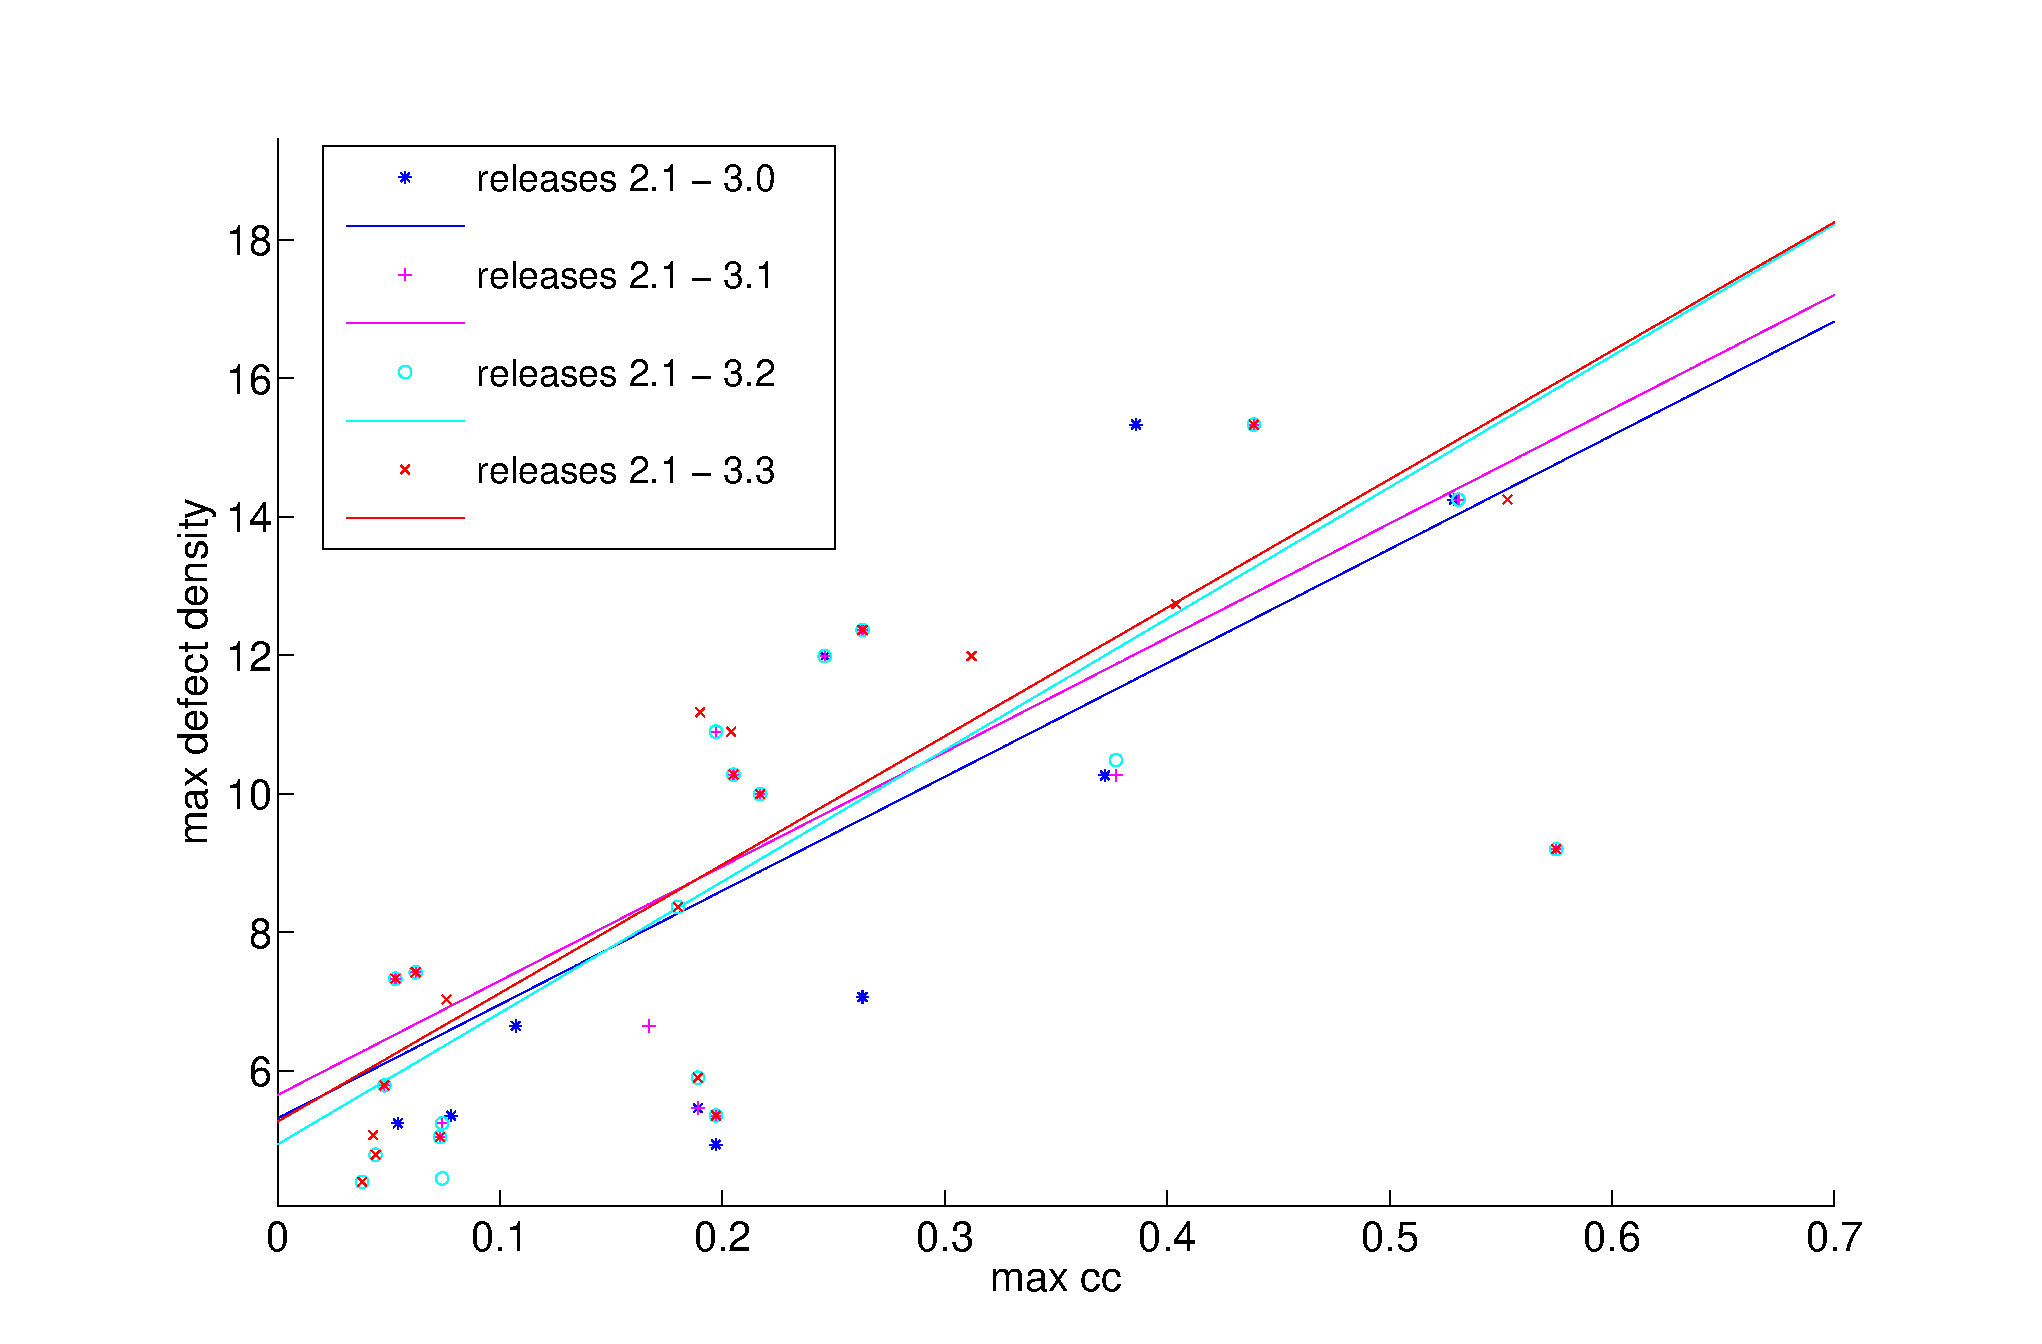
\includegraphics[width=\textwidth]{figure/nuovefig/cumulated_bug_cc_EC.eps}
    \label{cumulated_bug_cc_EC}
    \caption{Cumulated plots and fitting lines for the maximum defect density vs maximum clustering coefficient.}
\end{figure*}

    \begin{table}
    \centering
      \begin{tabular}{|l|c|c|c|}
      \hline
      \textbf{Releases} & $r$ & $\chi^2$ & $dof$  \\
      2.1 - 3-0 & 0.565 & 0.633 & 16  \\
      2.1 - 3.1 & 0.576 & 0.651  & 17  \\
      2.1 - 3.2 & 0.677 & 0.523 & 20 \\ 
      2.1 - 3.3 & 0.687 & 0.547 & 21 \\
      \hline
      \end{tabular}
       \caption{Fit data for the maximum defect density vs maximum clustering coefficient: correlation coefficient ($r$), 
      normalized Chi squared ($\chi^2$ ), and number of degrees of freedom ($dof$).}
\label{tab:max_abn-vs-maxcc}      
\end{table}
  


\section{Conclusions}
\label{Conclusions}
In this work we presented a longitudinal analysis on the evolution of a large software system with a focus on software defectiveness.
Through a complex network approach we were able to study the structure of 
the system by retrieving the community structure of the associated 
network. After retrieving the number of defects associated to the 
software network classes, we performed a topological analysis detecting the 
community structure. 
We found a power law relationship between the maximum values of the clustering coefficient, the average bug number and the division in communities of the software network. This lead to a linear relationship between the maximum values of clustering coefficient and of average bug number.
We show that such relationship can in principle be used as a predictor for the maximum value of the average bug number in future releases. 


\bibliographystyle{alpha} 

\bibliography{sigproc, reftest, ese_bibliography, sattose}


\end{document}


